% MathMode: full, MathRender: svg, MathDpi: 299, MathEmbedLimit: 524288, MathScale: 105, MathBaseline: 0, MathDocClass: [10pt]book, MathImgDir: math, MathLatex: latex, MathSvgFontFormat: "", MathSvgSharePaths: True, MathSvgPrecision: 3, Dvisvg: dvisvgm
\documentclass[10pt]{book}
% generated by Madoko, version 1.1.6
%mdk-data-line={1}
\newcommand\mdmathmode{full}
\newcommand\mdmathrender{svg}
\usepackage[heading-base={2},section-num={false},bib-label={true},fontspec={true}]{madoko2}
\usepackage[curve]{xypic}
\usepackage{amscd}
\usepackage[version=3]{mhchem}
\usepackage[UTF8]{xeCJK}
\usepackage{tikz}
\usepackage{pgfplots}
\usepackage{pgfplotstable}
\usepackage{pstricks}
\usepackage{pst-plot}

%mdk-data-line={24}
\usetikzlibrary{decorations.pathreplacing,decorations.pathmorphing}               
\begin{document}


\begin{mdSnippets}
%mdk-data-line={68}
%mdk-data-line={1312}
%mdk-begin-mathdefs
\newcommand{\infer}[3]{#1 \vdash #2\,:#3}

%mdk-data-line={1374}
\begin{mdDisplaySnippet}[0b7ef03f51a1cfe7642f8dec63290f9b]%mdk
\psset{unit=2cm} 
\begin{pspicture*}(-0.5,-1.5)(4,2)
  \psgrid[subgriddiv=5,gridcolor=black!20%
         ,gridlabels=0pt](1,0)(3,1.2)
  \psaxes{->}(0,0)(0,-1)(3.2,1.5)
  \uput[0](3.2,0){$x$}\uput[90](0,1.5){$f(x)$}
  \pscircle*[linecolor=red](! Euler 1){3pt}
  \psline[linecolor=red,linestyle=dashed]%
         (! Euler 0)(! Euler 1)
  \psline[linecolor=red,linewidth=0.2pt,arrowscale=2]%
         {->}(! Euler 1)(0, 1)
  \uput[-90](! Euler 0){\color{red}$e$}
  \pscircle*[linecolor=blue](1,0){3pt}
  \psplot[linewidth=1pt]{0.2}{3}{ x ln }
  \rput(1.6,-0.5){\color{blue}\fbox{$f(x)=\ln(x)$}} 
\end{pspicture*}\end{mdDisplaySnippet}%mdk
%mdk-data-line={1408}
\begin{mdDisplaySnippet}[c5f694d981cb7c9a0d22d7c345b23a6d]%mdk
%mdk-data-line={1412}
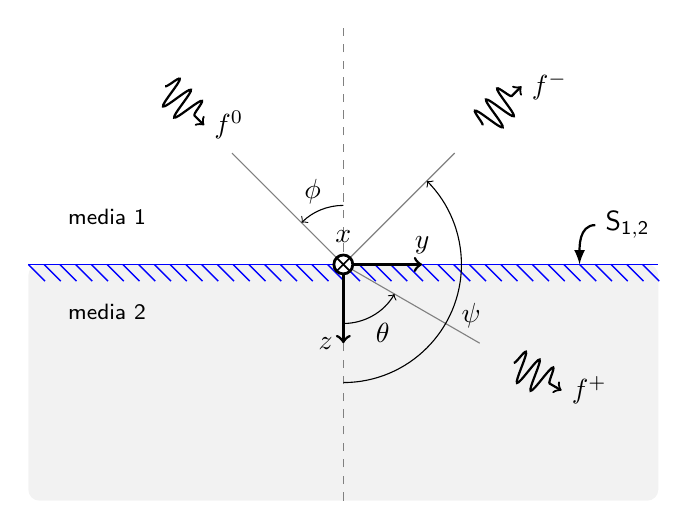
\begin{tikzpicture}[ 
    media/.style={font={\footnotesize\sffamily}},
    wave/.style={
        decorate,decoration={snake,post length=1.4mm,amplitude=2mm,
        segment length=2mm},thick},
    interface/.style={
        % The border decoration is a path replacing decorator. 
        % For the interface style we want to draw the original path.
        % The postaction option is therefore used to ensure that the
        % border decoration is drawn *after* the original path.
        postaction={draw,decorate,decoration={border,angle=-45,
                    amplitude=0.3cm,segment length=2mm}}},
    ]
    % Round rectangle
    \fill[gray!10,rounded corners] (-4,-3) rectangle (4,0);
    % Interface
    \draw[blue,line width=.5pt,interface](-4,0)--(4,0);
    % Vertical dashed line
    \draw[dashed,gray](0,-3)--(0,3);
    % Coordinates system
    \draw(0,0.15)node[above]{$x$};
    \draw[<->,line width=1pt] (1,0) node[above]{$y$}-|(0,-1) node[left]{$z$};
    % Incidence
    \draw[->,wave]
         (135:3.2cm)--(135:2.5cm)node[right]{$f^0$};
    \draw[gray](0:0cm)--(135:2cm);
    \path (0,0)++(113:1cm)node{$\phi$};
    \draw[->](0,0.75)arc(90:135:.75cm);
    % Transmission
    \draw[->,wave]
         (-30:2.5cm)--(-30:3.2cm)node[right]{$f^+$};
    \draw[gray](0:0cm)--(-30:2cm);
    \path (0,0)++(-60:1cm)node{$\theta$};
    \draw[->] (0,-0.75) arc (-90:-30:.75cm);
    % Reflection
    \draw[->,wave]
         (45:2.5cm)--(45:3.2cm)node[right]{$f^-$};
    \path (0,0)++(-22:1.75cm) node{$\psi$};
    \draw[gray](0:0cm)--(45:2cm);
    \draw[->] (0,-1.5)arc(-90:45:1.5cm);
    % Media names
    \path[media] (-3,.6)  node {media 1}
                 (-3,-.6) node {media 2};

    % $x$ axis
    \filldraw[fill=white,line width=1pt](0,0)circle(.12cm);
    \draw[line width=.6pt] (0,0)
                          +(-135:.12cm) -- +(45:.12cm)
                          +(-45:.12cm) -- +(135:.12cm);
    % Interface pointer
    \draw[-latex,thick](3.2,0.5)node[right]{$\mathsf{S_{1,2}}$}
         to[out=180,in=90] (3,0);
    % To-paths are really useful for drawing curved lines. The above
    % to path is equal to:
    %
    % \draw[-latex,thick](3.2,0.5)node[right]{$\mathsf{S_{1,2}}$}
    %      ..controls +(180:.2cm) and +(up:0.25cm) .. (3,0);
    % Internally the to path is translated to a similar bezier curve,
    % but the to path syntax hides the complexity from the user. 
\end{tikzpicture}\end{mdDisplaySnippet}%mdk
%mdk-data-line={1474}
\begin{mdDisplaySnippet}[978a2cac0b346978e36123174d88a38e]%mdk
%mdk-data-line={1479}
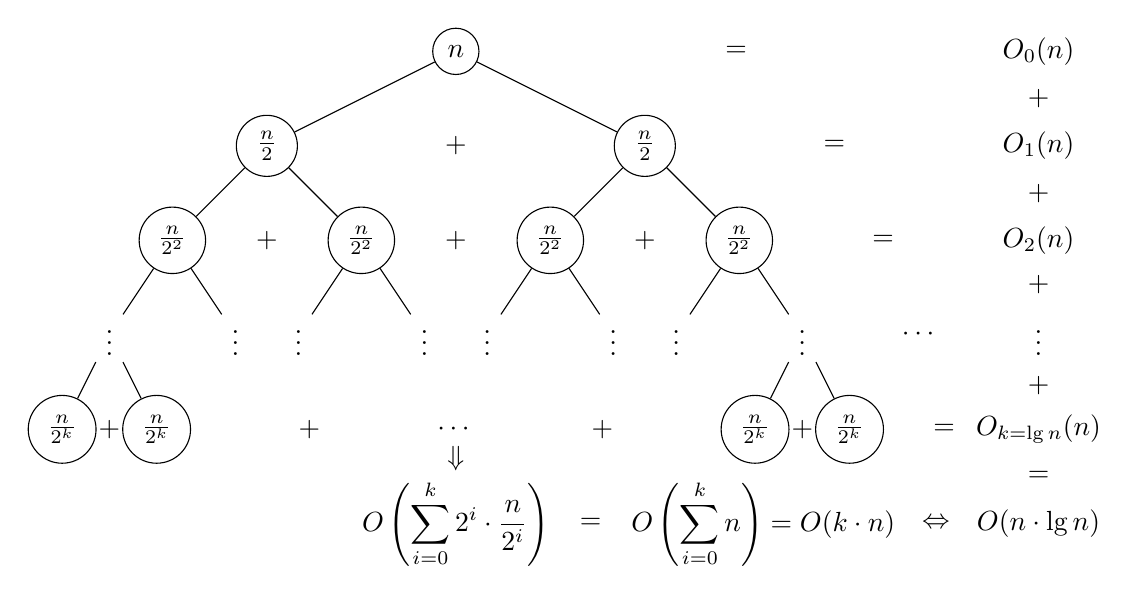
\begin{tikzpicture}[scale=0.8,level/.style={sibling distance=60mm/#1}]
\node [circle,draw] (z){$n$}
  child {node [circle,draw] (a) {$\frac{n}{2}$}
    child {node [circle,draw] (b) {$\frac{n}{2^2}$}
      child {node {$\vdots$}
        child {node [circle,draw] (d) {$\frac{n}{2^k}$}}
        child {node [circle,draw] (e) {$\frac{n}{2^k}$}}
      } 
      child {node {$\vdots$}}
    }
    child {node [circle,draw] (g) {$\frac{n}{2^2}$}
      child {node {$\vdots$}}
      child {node {$\vdots$}}
    }
  }
  child {node [circle,draw] (j) {$\frac{n}{2}$}
    child {node [circle,draw] (k) {$\frac{n}{2^2}$}
      child {node {$\vdots$}}
      child {node {$\vdots$}}
    }
  child {node [circle,draw] (l) {$\frac{n}{2^2}$}
    child {node {$\vdots$}}
    child {node (c){$\vdots$}
      child {node [circle,draw] (o) {$\frac{n}{2^k}$}}
      child {node [circle,draw] (p) {$\frac{n}{2^k}$}
        child [grow=right] {node (q) {$=$} edge from parent[draw=none]
          child [grow=right] {node (q) {$O_{k = \lg n}(n)$} edge from parent[draw=none]
            child [grow=up] {node (r) {$\vdots$} edge from parent[draw=none]
              child [grow=up] {node (s) {$O_2(n)$} edge from parent[draw=none]
                child [grow=up] {node (t) {$O_1(n)$} edge from parent[draw=none]
                  child [grow=up] {node (u) {$O_0(n)$} edge from parent[draw=none]}
                }
              }
            }
            child [grow=down] {node (v) {$O(n \cdot \lg n)$}edge from parent[draw=none]}
          }
        }
      }
    }
  }
};
\path (a) -- (j) node [midway] {+};
\path (b) -- (g) node [midway] {+};
\path (k) -- (l) node [midway] {+};
\path (k) -- (g) node [midway] {+};
\path (d) -- (e) node [midway] {+};
\path (o) -- (p) node [midway] {+};
\path (o) -- (e) node (x) [midway] {$\cdots$}
  child [grow=down] {
    node (y) {$O\left(\displaystyle\sum_{i = 0}^k 2^i \cdot \frac{n}{2^i}\right)$}
    edge from parent[draw=none]
  };
\path (q) -- (r) node [midway] {+};
\path (s) -- (r) node [midway] {+};
\path (s) -- (t) node [midway] {+};
\path (s) -- (l) node [midway] {=};
\path (t) -- (u) node [midway] {+};
\path (z) -- (u) node [midway] {=};
\path (j) -- (t) node [midway] {=};
\path (y) -- (x) node [midway] {$\Downarrow$};
\path (v) -- (y)
  node (w) [midway] {$O\left(\displaystyle\sum_{i = 0}^k n\right) = O(k \cdot n)$};
\path (q) -- (v) node [midway] {=};
\path (e) -- (x) node [midway] {+};
\path (o) -- (x) node [midway] {+};
\path (y) -- (w) node [midway] {$=$};
\path (v) -- (w) node [midway] {$\Leftrightarrow$};
\path (r) -- (c) node [midway] {$\cdots$};
\end{tikzpicture}\end{mdDisplaySnippet}%mdk
%mdk-data-line={0;out\prelude.mdk:536}
\begin{mdDisplaySnippet}[56acf2e836f837d085c39c59a579249e]%mdk
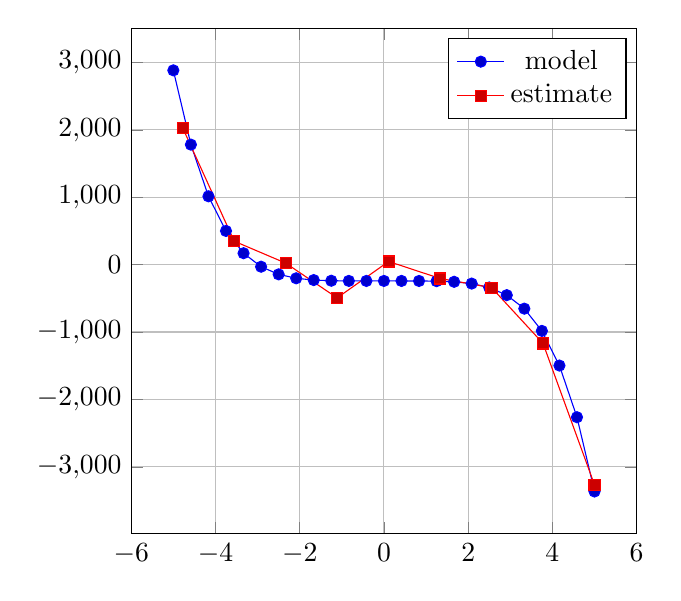
\begin{tikzpicture}
\begin{axis}[
  height=8cm,
  width=8cm,
  grid=major,
]
% math plot
\addplot {-x^5 - 242}; 
\addlegendentry{model}
% data plot
\addplot coordinates {
(-4.77778,2027.60977)
(-3.55556,347.84069)
(-2.33333,22.58953)
(-1.11111,-493.50066)
(0.11111,46.66082)
(1.33333,-205.56286)
(2.55556,-341.40638)
(3.77778,-1169.24780)
(5.00000,-3269.56775)
};
\addlegendentry{estimate}
\end{axis}
\end{tikzpicture}\end{mdDisplaySnippet}%mdk
%mdk-data-line={1593}
\begin{mdDisplaySnippet}[b1681e56ede4eea7f309c3a95446c29d]%mdk
%mdk-data-line={1602}
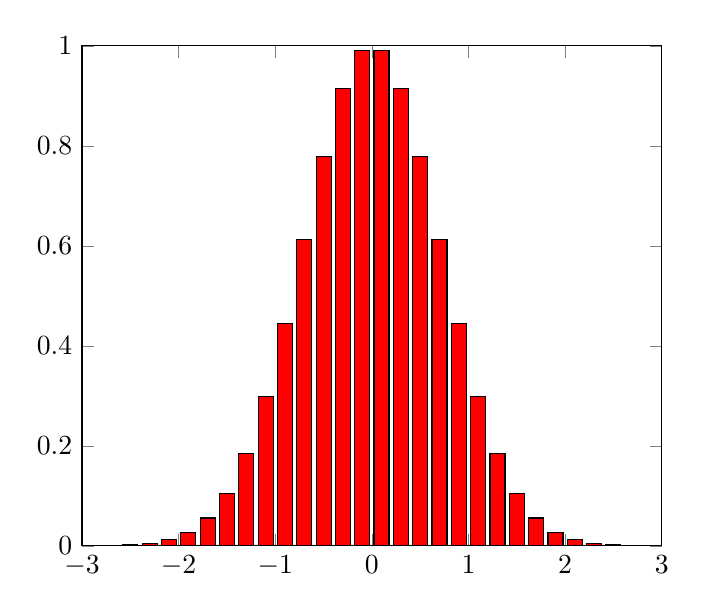
\begin{tikzpicture}
\begin{axis}[%
scale only axis,
height=2.5in,
xmin=-3, xmax=3,
ymin=0, ymax=1,
axis on top]
\addplot[
  ybar,
  bar width=0.075in, 
  bar shift=0in,
  fill=red,
  draw=black] 
  plot coordinates{ 
    (-2.9,0.00022263) (-2.7,0.000682328) (-2.5,0.00193045) (-2.3,0.00504176)
    (-2.1,0.0121552) (-1.9,0.0270518) (-1.7,0.0555762) (-1.5,0.105399)
    (-1.3,0.18452) (-1.1,0.298197) (-0.9,0.444858) (-0.7,0.612626)
    (-0.5,0.778801) (-0.3,0.913931) (-0.1,0.99005) (0.1,0.99005)
    (0.3,0.913931) (0.5,0.778801) (0.7,0.612626) (0.9,0.444858) 
    (1.1,0.298197) (1.3,0.18452) (1.5,0.105399) (1.7,0.0555762)
    (1.9,0.0270518) (2.1,0.0121552) (2.3,0.00504176) (2.5,0.00193045)
    (2.7,0.000682328) (2.9,0.00022263)
  };
\end{axis}
\end{tikzpicture}\end{mdDisplaySnippet}%mdk
\begin{mdDisplaySnippet}[aff15b1e067a1f01f390ed28d915d560]%mdk
%mdk-data-line={1631}
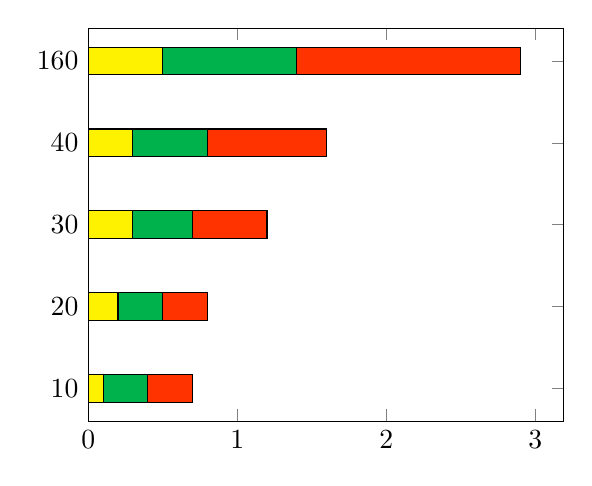
\begin{tikzpicture}
\pgfplotstableread{ % Read the data into a table macro
Label   First   Second  Third
10      0.1     0.3     0.3
20      0.2     0.3     0.3
30      0.3     0.4     0.5
40      0.3     0.5     0.8
160     0.5     0.9     1.5
}\datatable
\begin{axis}[
    width=3in,
    xbar stacked,   % Stacked horizontal bars
    xmin=0,         % Start x axis at 0
    ytick=data,     % Use as many tick labels as y coordinates
    yticklabels from table={\datatable}{Label}  % Get the labels from the Label column of the \datatable
]
\addplot [fill=yellow] table [x=First, y expr=\coordindex] {\datatable};    % Plot the "First" column against the data index
\addplot [fill=green!70!blue]table [x=Second, y expr=\coordindex] {\datatable};
\addplot [fill=red!80!yellow] table [x=Third, y expr=\coordindex] {\datatable};
\end{axis}
\end{tikzpicture}\end{mdDisplaySnippet}%mdk
%mdk-data-line={3216}

\end{mdSnippets}

\end{document}
